\documentclass[a4paper,12pt]{article}
\usepackage[utf8]{inputenc}

\usepackage[utf8]{inputenc}
\usepackage[T2A]{fontenc}
\usepackage[english,russian]{babel}
\usepackage{amsthm}
\usepackage{amsmath}
\usepackage{amssymb}
\usepackage{tikz}
\usepackage{textcomp}
\usepackage{marvosym}
\usepackage{ esint }
\usepackage{mathtext}
\usepackage{siunitx} % Required for alignment
\usepackage{subfigure}
\usepackage{multirow}
\usepackage{rotating}
\usepackage{afterpage}
\usepackage[arrowdel]{physics}
\usepackage{booktabs}
\setlength{\topmargin}{-0.5in}
\setlength{\textheight}{9.1in}
\setlength{\oddsidemargin}{-0.4in}
\setlength{\evensidemargin}{-0.4in}
\setlength{\textwidth}{7in}
\setlength{\parindent}{0ex}
\setlength{\parskip}{1ex}
\newcommand{\ndiv}{\hspace{-4pt}\not|\hspace{2pt}}
\usepackage{graphicx}
\usepackage{float}
\usepackage{wrapfig}
\usepackage{pgfplots}
\usepackage{caption}
\pgfplotsset{compat=1.16}
\graphicspath{ {./images/} }
\usepackage{graphicx}
\RequirePackage{caption}
\DeclareCaptionLabelSeparator{defffis}{ — }
\captionsetup{justification=centering,labelsep=defffis}
\usepackage{caption} \captionsetup[table]{labelsep=endash,justification=justified,singlelinecheck=false,font=normalsize}
\usepackage{amsfonts,mathtools}

\title{Лабораторная работа № 5.10.1\\Электронный парамагнитный резонанс}
\author{Илья Прамский}
\date{Октябрь 2024}

\begin{document}
\maketitle
\newpage
\section{Теоретическая справка}

Энергетический уровень электрона в присутствии магнитного поля с индукцией B расщепляется на два подуровня, расстояние между которыми равно
\begin{equation}
\Delta E = E_2 - E_1 - 2 \mu B
\end{equation}
Где $\mu$ - абсолютная величина проекции магнитного момента на направление поля.

Резонансное значение частоты(частота электромагнитного поля, необходимая для перехода между уровнями) определяется из формулы 
\begin{equation}
\hbar \omega_0 = \Delta E
\end{equation}
Возбуждение электронных резонансных переходов электромагнитным полем, имеющим частоту, определяемую формулой (2), носит название электронного парамагнитного резонанса (ЭПР).

Связь магнитного момента электрона с его механическим моментом определяется с помощью формулы
\begin{equation}
\textbf{$\mu$} = \gamma \textbf{M}
\end{equation}
Из соотношений выше можно получить выражение для g-фактора
\begin{equation}
g = \frac{\hbar \omega_0}{\mu_{\text{Б}} B}
\end{equation}

\begin{figure}[H]
\centering
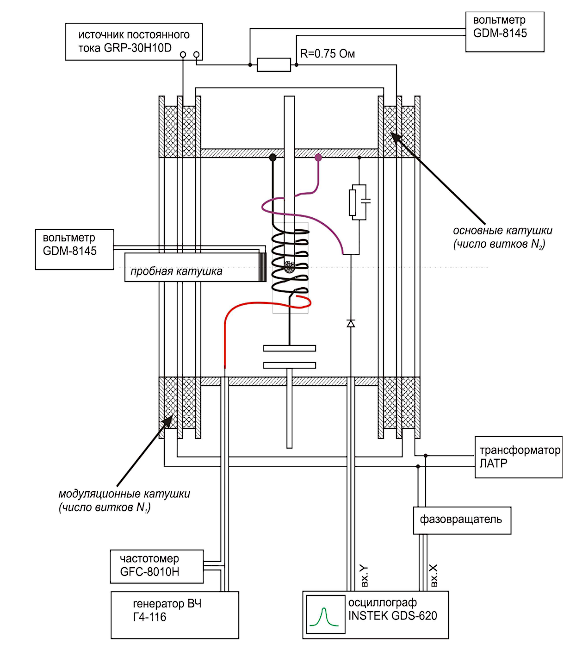
\includegraphics[scale=0.8]{scheme.png}
\end{figure}

Показания лампового милливольтметра и величина магнитного поля связаны через соотношение
\begin{equation}
V = n B_0 S \omega_\simeq
\end{equation}
где n - число витков и S - площадь сечения пробной катушки, $\omega_\simeq$ - угловая частота переменного тока.

\section{Ход работы}
\subsection*{Получение сигнала ЭПР на свободном радикале ДФПГ и измерение g-фактора электрона}
Значение частоты резонанса $f_\text{рез} = 163,15 \pm 0,01$ МГц.

$f_\text{мод} = 1$ кГц, $m = 20\%$

Значение напряжения в цепи основных катушек при резонансном поглощении $U_0 = 129,8 \pm 0,1$ мВ.

Показания лампового милливольтметра при настройке установки на вычисление магнитного поля по формуле (5):

Спереди $U_1 = 14,5 \pm 0,1$ мВ;

Сзади $U_2 = 14,9 \pm 0,1$ мВ;

Получается $V = 14,7 \pm 0,1$ мВ.

Характеристики пробной катушки: $D = 15,2 \pm 0,1$ мм. $n_0 = 45$. Также $\omega_\simeq = 2 \pi \cdot 50$

По формуле (5)
\[B_0 = \frac{4V}{n_0 \omega_\simeq \pi D^2} = 5,73 \pm 0,08 \text{мТл}\]

Тогда найдём g-фактор, зная $\mu_\text{Б} = 0,927 \cdot 10^{-23}$ Дж/Тл
\[g = 2,03 \pm 0,03\]

\subsection*{Измерение ширины линии ЭПР}
Для начала найдём магнитное поле модуляции при помощи формулы (5), не забыв учесть, что вольтметр в данном случае показывает эффективное значение напряжение, а не максимальное

Спереди $U_1 = 1,52 \pm 0,1$ мВ;

Сзади $U_2 = 1,34 \pm 0,1$ мВ;

$V = 1,43 \pm 0,3$ мВ.

\[B_\text{мод} = \frac{4 \cdot \sqrt{2}V}{n_0 \omega_\simeq \pi D^2} = 0,79 \pm 0,17 \text{мТл}\]
Ширина по X соответствует $2B_\text{мод}$.

\begin{figure}[H]
\centering
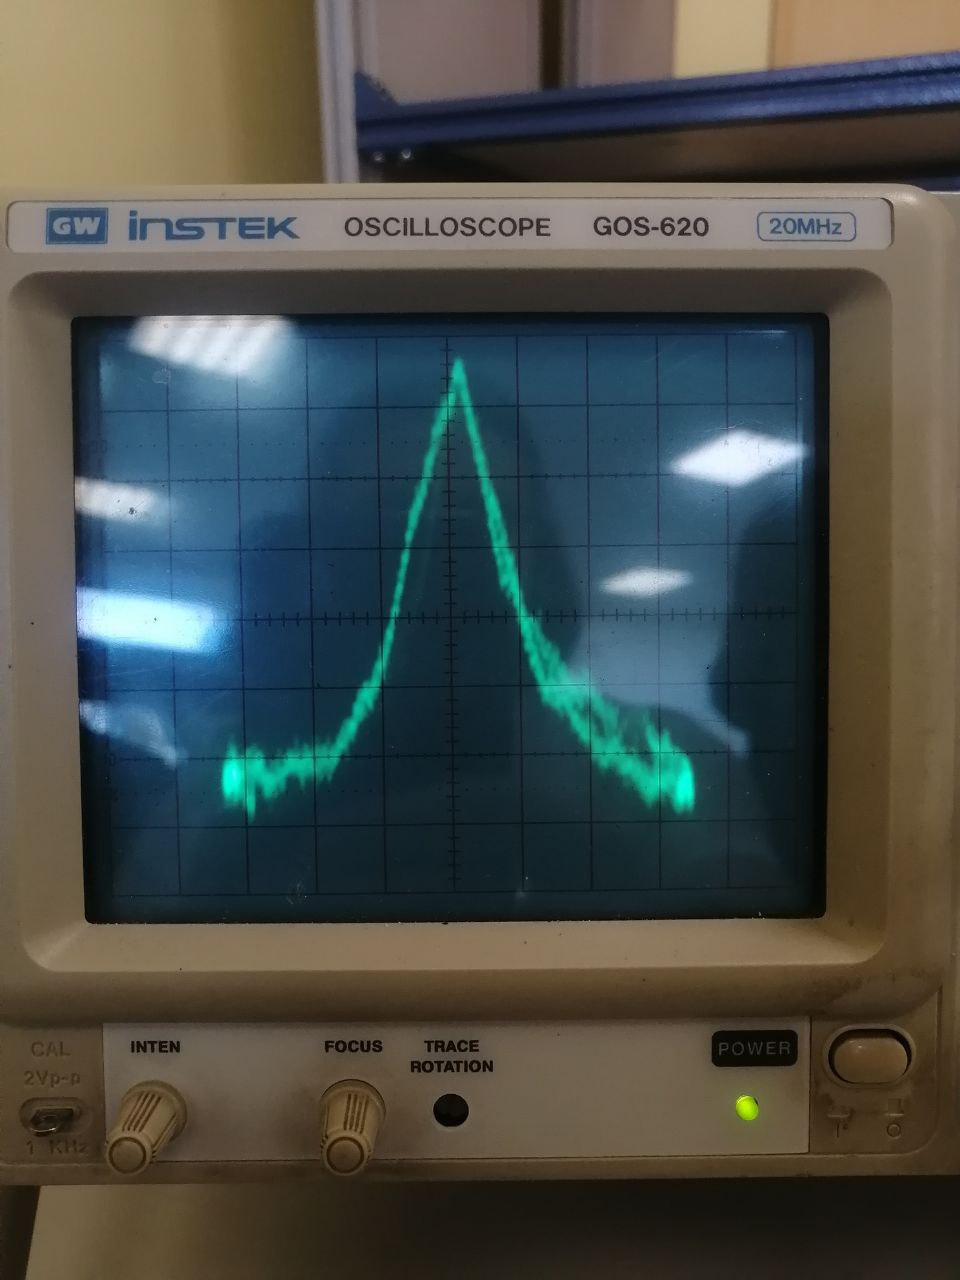
\includegraphics[scale=0.2]{line1.jpg}
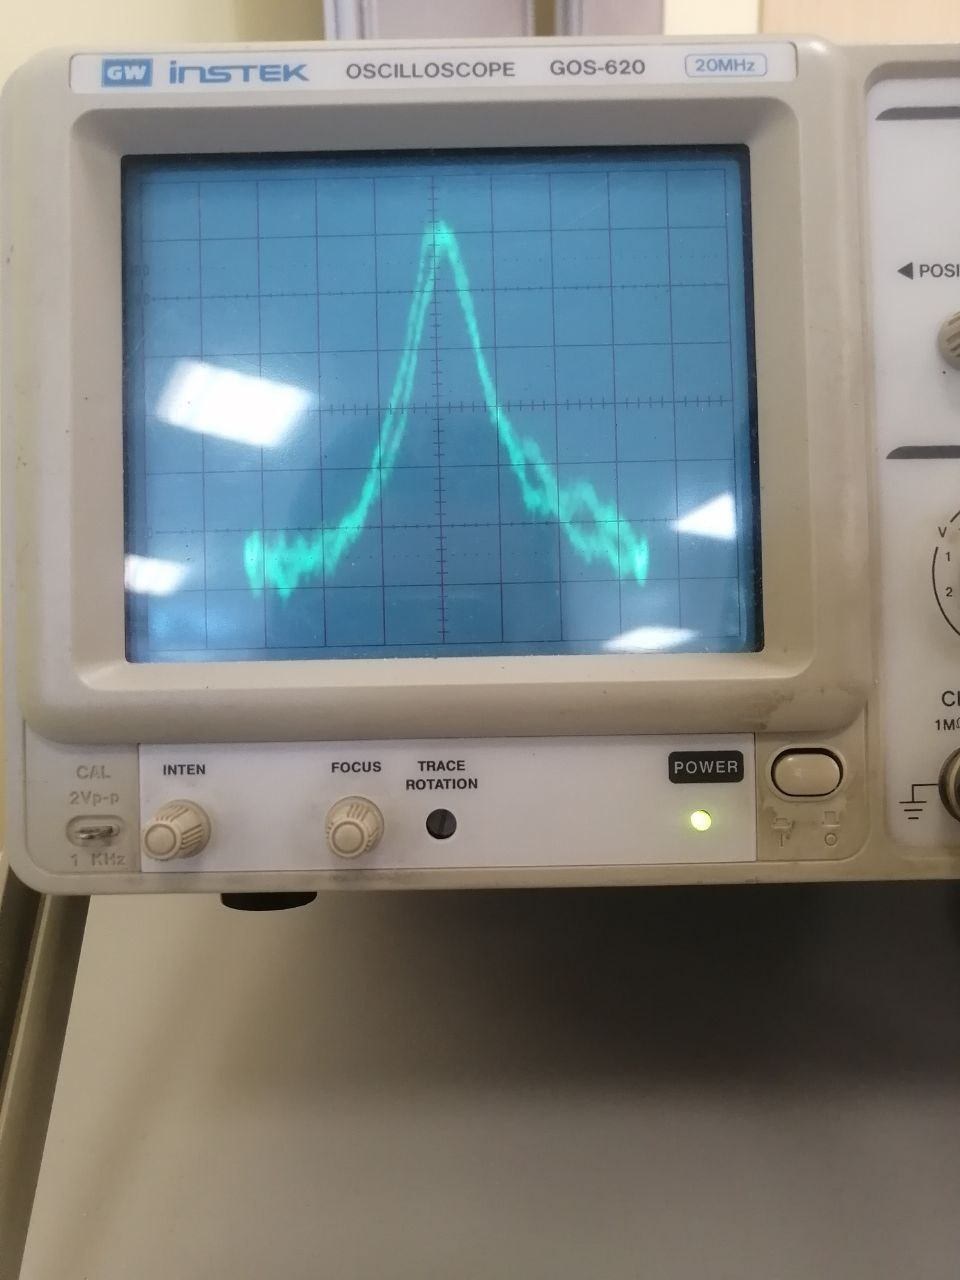
\includegraphics[scale=0.2]{line2.jpg}
\end{figure}
Из картины на осциллографе видно, что ширина по $X \approx 6$ клетки, значит одна клетка соответствует $\frac{2 B_\text{мод}}{6}$.

Тогда ширина $\Delta B = 0,9 \cdot \frac{2 B_\text{мод}}{6} = 0,24 \pm 0,05$ мТл.

\section{Вывод}
В ходе работы был измерен g-фактор электрона. Получилось $g = 2,03 \pm 0,03$, когда справочное значение $g_\text{ист} = 2$. Также было получено значение ширины линии ЭПР $\Delta B = 0,24 \pm 0,05$ мТл.
\end{document}